\documentclass[fleqn]{beamer}
%\usepackage{xkeyval}
%\usepackage{todonotes}
%\presetkeys{todonotes}{inline}{}
\usepackage{xcolor}
\usepackage{tcolorbox}
%\usepackage{lipsum}
%\usepackage{xargs}
%\usepackage[pdftex,dvipsnames]{xcolor}  % Coloured text etc.

\usepackage{tabularx}
\usepackage{booktabs}
\usepackage{colortbl}
\usepackage{tikz}
\usetikzlibrary{calc}
\pgfdeclarelayer{background}
\pgfdeclarelayer{foreground}
\pgfsetlayers{background,main,foreground}
%\setbeamertemplate{background canvas}[vertical shading]%
%  [top=blue!1,bottom=blue!30]
\setbeamertemplate{navigation symbols}{}
\newcommand*\up{\textcolor{green}{%
  \ensuremath{\blacktriangle}}}
\newcommand*\down{\textcolor{red}{%
  \ensuremath{\blacktriangledown}}}
\newcommand*\const{\textcolor{darkgray}%
  {\textbf{--}}}

\newcounter{todo}
\newtcbox{\mytodobox}{colback=orange,colframe=orange!75!black}

 \newcommand\todo[1]{%
     \refstepcounter{todo} 
    \mytodobox{\hypertarget{todo\thetodo}{#1}}
     \addcontentsline{tod}{subsection}{\protect\hyperlink{todo\thetodo}{\thetodo~#1}\par} 
 }%

\makeatletter
\newcommand\listoftodos{%
    \@starttoc{tod}}
\makeatother

\usepackage{graphicx,ksu,url}
\usepackage{amsmath}
% Use Times for math font and text font.
\RequirePackage[T1]{fontenc}
%\RequirePackage{txfonts}
% bold math must be loaded after Times font
\usepackage{bm}
\usepackage{booktabs} % nice rules (thick lines) for tables
\usepackage{microtype} % improves typography for PDF
\usepackage{xcolor} % Allows colors in fonts
\usepackage{tikz} % Allows creation of tikz pictures
\usepackage{verbatim}
\usepackage{fancyvrb}
\usepackage{mathalfa}
\usepackage{mathrsfs}
\DeclareMathOperator*{\argmin}{argmin}
\DeclareMathAlphabet{\mathpzc}{OT1}{pzc}{m}{bf}
\renewcommand{\vec}[1]{\bm{#1}} %vector is bold italic
\newcommand{\vd}{\bm{\cdot}} % slightly bold vector dot
\newcommand{\grad}{\vec{\nabla}} % gradient
\newcommand{\ud}{\mathop{}\!\mathrm{d}} % upright derivative symbol
\graphicspath{{../data/images/}}

\usetikzlibrary{arrows,shapes}
\usetikzlibrary{decorations.pathreplacing,matrix, positioning}
\setlength\intextsep{1\baselineskip plus 3pt minus 2 pt}
\usepackage{minted} % Allows printing of python (or other) code
\newminted{python}{fontsize=\scriptsize, 
    linenos,
    numbersep=8pt,
    gobble=4,
    frame=lines,
    bgcolor=bg,
    framesep=3mm}

% The title of the presentation:
%  - first a short version which is visible at the bottom of each slide;
%  - second the full title shown on the title slide;
\title[]{
    Analysis of the LRA Reactor Benchmark Using Dynamic Mode Decomposition}

% Optional: a subtitle to be displayed on the title slide
%\subtitle{Show where you're from}

% The author(s) of the presentation:
%  - again first a short version to be displayed at the bottom;
%  - next the full list of authors, which may include contact information;
\author[]{
	Dr. Mohammad Abdo \\
    Rabab Elzohery \\
    Prof. Jeremy Roberts}

% The institute:
%  - to start the name of the university as displayed on the top of each slide
%    this can be adjusted such that you can also create a Dutch version
%  - next the institute information as displayed on the title slide
\institute[Kansas State University]{
    Mechanical and Nuclear Engineering \\
    Kansas State University}

% Add a date and possibly the name of the event to the slides
%  - again first a short version to be shown at the bottom of each slide
%  - second the full date and event name for the title slide

\date[]{\emph{\textbf{2018 ANS Winter Meeting and Nuclear Technology Expo, "Joining Forces to Advance Nuclear"}}
    November 11-15- 2018}

\begin{document}
    % These two commands allow bonus slides at the end
    % The bonus slides will not be numbered
    \newcommand{\beginbackup}{
        \newcounter{framenumbervorappendix}
        \setcounter{framenumbervorappendix}{\value{framenumber}}
    }
    \newcommand{\backupend}{
        \addtocounter{framenumbervorappendix}{-\value{framenumber}}
        \addtocounter{framenumber}{\value{framenumbervorappendix}} 
    }
    
    \begin{frame}
        \titlepage
    \end{frame}
    

    \section{Background and Motivation}
    
    \begin{frame}
        \frametitle{LRA Benchmark}
\textbf{Write something about LRA and a slide or two about Detran}       
\begin{itemize}
       \item 
       \item 
   
       \item  
%         
    \item 
    
    \item 
       
  
       \end{itemize}
    \end{frame}

    
   % \section{Reduced Order Models} % new section title
    \begin{frame}
    \frametitle{Reduced Order Modeling}

    \begin{itemize}
    %\item Reduced order models are approximation of the original expensive model, that could represent the model in terms of a lower number of inputs.
   \begin{block}{ROM}
%\begin{equation*}
\centering
$\vec{f}(\vec{x})\approx \vec{g}(\mathcal{M}(\vec{x})); \ \ \vec{x} \subseteq \mathbb{R}^n, \mathcal{M}(\vec{x}) \in \mathbb{R}^{r_x}; r_x << n$
%    \end{equation*}
\end{block}

    \item This is usually done by projecting the problem high dimensional space onto a lower space that captures most of the data variance (i.e POD).
    
    \item In this work, Dynamic Mode Decomposition (DMD) was used to construct a data-driven surrogate model. 
    \end{itemize}
    \end{frame}
    \section{Actual Model Description}

    \begin{frame}
        \frametitle{Physical Model}
        \begin{columns}[c]
            \begin{column}{0.7\textwidth} 
\begin{figure}
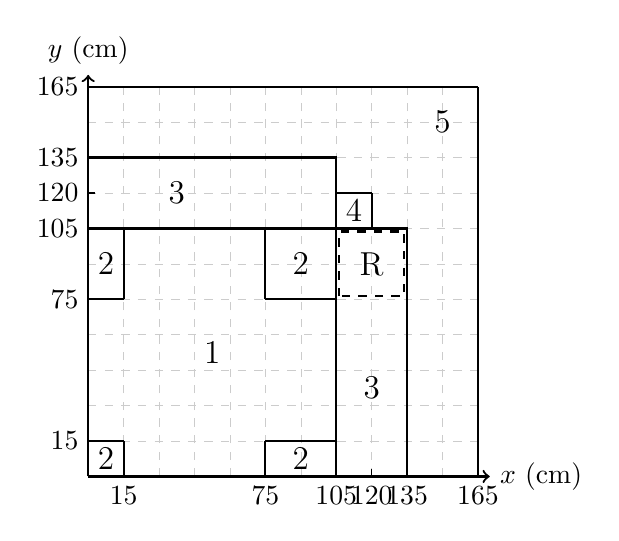
\begin{tikzpicture}[scale=.3]

\begin{scope}<->;

% GRID
  \draw[step=1.5cm,gray,very thin, dashed,opacity=0.4] (0, 0) grid (16.5,16.5);

% AXES
  \draw[black, thick, ->] (0, 0) -- (17,  0) node[right] {$x$ (cm)};
  \draw[black, thick, ->] (0, 0) -- ( 0, 17) node[above] {$y$ (cm)};

% Material 1 regions 

  \node[font=\large] at (5.25, 5.25) {1};
  
% Material 2 regions
  \draw[black, thick] (0, 1.5) -- (1.5, 1.5);
  \draw[black, thick] (1.5, 0) -- (1.5, 1.5);
  \node[font=\large] at (0.75, 0.75) {2};
  
  \draw[black, thick] ( 7.5, 0.0) -- ( 7.5, 1.5);
  \draw[black, thick] (10.5, 0.0) -- (10.5, 1.5);
  \draw[black, thick] ( 7.5, 1.5) -- (10.5, 1.5);
  \node[font=\large] at (9.0, 0.75) {2};

  \draw[black, thick] ( 0.0,  7.5) -- ( 1.5,  7.5);
  \draw[black, thick] ( 0.0, 10.5) -- ( 1.5, 10.5);
  \draw[black, thick] ( 1.5,  7.5) -- ( 1.5, 10.5);
  \node[font=\large] at ( 0.75, 9.0) {2};
  
  \draw[black, thick] ( 7.5,  7.5) -- ( 7.5, 10.5);
  \draw[black, thick] ( 7.5,  7.5) -- (10.5,  7.5);
  \draw[black, thick] (10.5, 10.5) -- ( 7.5, 10.5);
  \draw[black, thick] (10.5, 10.5) -- (10.5,  7.5);
  \node[font=\large] at ( 9.0, 9.0) {2};

% Material 3 regions
  \draw[black, thick] (10.5,  0.0) -- (10.5, 10.5) -- (13.5, 10.5) --  (13.5,  0.0) -- (10.5,  0.0);
  \node[font=\large] at ( 12.0, 3.75) {3}; 
  \draw[black, thick] (0.0, 10.5) -- (10.5, 10.5) -- (10.5, 13.5) -- (0.0, 13.5) --  (0.0, 10.5);
  \node[font=\large] at ( 3.75, 12.0) {3}; 
  
% Material 4 regions  
  \draw[black, thick] ( 12,  12) -- ( 12, 10.5) -- (10.5, 10.5) -- (10.5,  12) -- ( 12,  12);
  \node[font=\large] at ( 11.25,11.25) {4};

   
% Material 5 regions
  \draw[black, thick] ( 16.5,  0.0) -- (16.5, 16.5);
  \draw[black, thick] (  0.0, 16.5) -- (16.5, 16.5);
  \node[font=\large] at (15.0, 15.0) {5};
 
% Perturbed regions
  \def\eps{0.125}
  \draw[black, thick, dashed] (10.5+\eps, 7.5+\eps) -- (10.5+\eps, 10.5-\eps) -- (13.5-\eps, 10.5-\eps) -- (13.5-\eps, 7.5+\eps) --  (10.5+\eps, 7.5+\eps);

  %\draw[black, thick] ( 12,  12) -- (10.5,  12);
  %\draw[black, thick] (10.5, 10.5) -- ( 12, 10.5);
  %\draw[black, thick] (10.5, 10.5) -- (10.5,  12);
  \node[font=\large] at (12,9) {R};
 
% ticks
  \foreach \x/\xtext in {15, 75, 105, 120, 135, 165}
      \draw[black,xshift=0.1*\x cm] (0,.3) -- (0,0) node[below] {$\xtext$};
  \foreach \y/\ytext in {15, 75, 105, 120, 135, 165}
      \draw[black,yshift=0.1*\y cm] (.3,0) -- (0,0) node[left] {$\ytext$};
\end{scope}
\end{tikzpicture}
\end{figure}
            \end{column}            
            \begin{column}{0.4\textwidth} 
                             \begin{block}{Model Description}              
 \begin{itemize}     
                    \item Super Prompt-critical Transient. 
                    \item 2D Diffusion.
                    \item Adiabatic Heatup and Doppler Feedback in thermal reactor.
                    
                    \end{itemize}
                \end{block}
            \end{column}
        \end{columns}
    \end{frame}
    \begin{frame}
    \frametitle{Governing Equations}
\begin{block}{2D Diffusion with two Delayed Neutron Precursor groups.}

	\begin{align*}
	\label{eq:Diffusion}
	& \nabla D_1(\vec{x},t)\nabla \phi_1(\vec{x},t)-[\Sigma_{a1}(\vec{x},t)+\Sigma_{1\rightarrow2}(\vec{x},t)]\phi_1(\vec{x},t)\\
	& +\nu( 1- \beta )[\Sigma_{f1}(\vec{x},t)\phi_1(\vec{x},t)+\Sigma_{f2}(\vec{x},t)\phi_2(\vec{x},t)]\\
	& +\Sigma_{i=1}^{2}\lambda_i c_i (\vec{x},t)=\frac{1}{v_1}\frac{\partial}{\partial t}\phi_1(\vec{x},t).\\
	& \nabla D_2(\vec{x},t)\nabla \phi_2(\vec{x},t)-\Sigma_{a2}(\vec{x},t)\phi_2(\vec{x},t)+\Sigma_{1\rightarrow2}(\vec{x},t)\phi_1(\vec{x},t)\\
	& =\frac{1}{v_2}\frac{\partial}{\partial t}\phi_2(\vec{x},t).\\
	& \nu\beta_i[\Sigma_{f1}(\vec{x},t)\phi_1(\vec{x},t)+\Sigma_{f2}(\vec{x},t)\phi_2(\vec{x},t)]-\lambda_ic_i(\vec{x},t)\\
	&=\frac{\partial}{\partial t}c_i(\vec{x},t), \ i=1,2.
	\end{align*}
\end{block}
\end{frame}
\begin{frame}
\begin{block}{Adiabatic Heatup}
\begin{equation*}
\alpha[\Sigma_{f1}(\vec{x},t)\phi_1(\vec{x},t)+\Sigma_{f2}(\vec{x},t)\phi_2(\vec{x},t)]=\frac{\partial}{\partial t}T(\vec{x},t).
\end{equation*}
\end{block}

\begin{block}{Doppler Feedback}
\begin{equation*}
\Sigma_{a1}(\vec{x},t) = \Sigma_{a2}(\vec{x},t=0)[1+\gamma(\sqrt(T(\vec{x},t))-\sqrt(T_0))].
\end{equation*}
\end{block}

\begin{block}{Power}
\begin{equation*}
P(\vec{x},t)=\varepsilon [\Sigma_{f1}(\vec{x},t)\phi_1(\vec{x},t)+\Sigma_{f2}(\vec{x},t)\phi_2(\vec{x},t)].
\end{equation*}
\end{block}
\end{frame}
% * <mgabdo@ksu.edu> 2018-03-28T13:53:50.537Z:
%
% ^.
\section{Dynamic Mode Decomposition}
\begin{frame}
\frametitle{DMD Overview}
\begin {itemize}
\item DMD was first used by Schmid in 2008, in fluid dynamics \cite{schmid08}.
\item It is used to explore the behavior of dynamical systems.
\item  It can be viewed as a PCA (spatial domain) + DFT (frequency domain).
% \item  It can be viewed as a combination of a PCA in the spatial domain and Discrete Fourier Transform (DFT) in the frequency domain.

\end{itemize}
\end{frame}
\begin{frame}
\frametitle {DMD Methodology}
Consider a sequential dataset ($\mathbf{X} \subseteq \mathbb{R}^{n\times m}$) spaced by $\Delta t$.
     \begin{figure}[!htb]
     \centering
  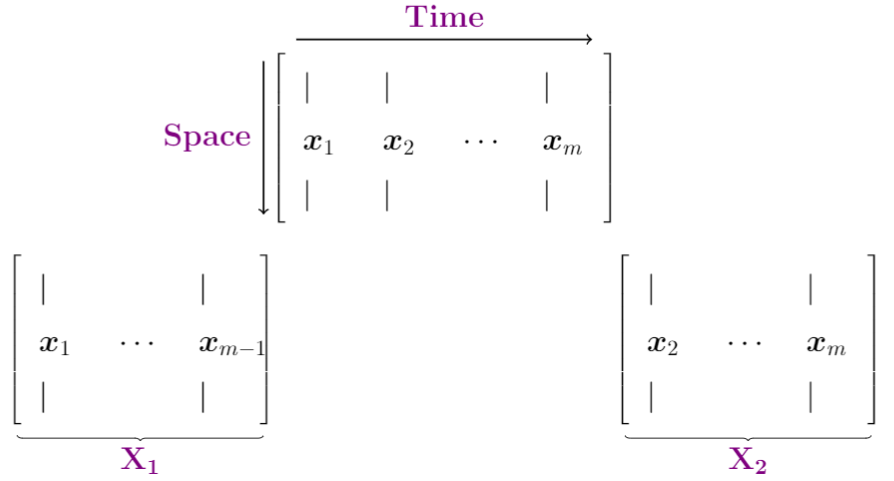
\includegraphics[scale=0.29]{DATA.png}
  \label{fig:data_matrix}
\end{figure} 
\begin{block}{}
\small{\textbf{Assumption}: With sufficiently small $\Delta t$, there is a linear time marching operator $\mathbf{A}$ that approximates the system's dynamic, such that;} 
\centering
$
         \mathbf{X_2} \approx  \tikz[baseline]{\node[draw=purple,anchor=base,
circle,inner xsep=-2pt,inner ysep=3pt] {$\mathbf{A}$}} \mathbf{X_1}
$

\end{block}
\end{frame}

\begin{frame}
\frametitle{DMD Methodology}
\begin{block}{}
$\mathbf{A}$ is the operator that best fits the data in a least-squares sense;
\centering
$\mathbf{A}=\argmin\limits_{\mathbf{A}}\|\mathbf{X_{2}} -\mathbf{AX_{1}}\|_F \, ,
$\\
${\mathbf{A}\approx\mathbf{X_2}\mathbf{X_1^{\dagger}}} $
\end{block}
\begin{block}{}
In practice, $\mathbf{A}$  is very large $\to$ DMD tries to approximate its eigenpairs.
\end{block}
\begin{block}{}
The Singular Value Decomposition(\textbf{SVD}) is computed for $\mathbf{X_1}$;
\centering
${\mathbf{X_1} = \mathbf{U}\boldsymbol{\Sigma}\mathbf{V^{H}} }$
\end{block}
\end{frame}

  \begin{frame}
  \frametitle{Singular Value Decomposition}
\begin{block}{}
The SVD is exploited to reveal the low dimensional structure in the data by keeping the first r singular values that recovers most of the data variance;\\
\centering
${\mathbf{X_1} \approx \mathbf{U_r}\boldsymbol{\Sigma}_{\mathbf{r}}\mathbf{V_r^{H}} }$
\end{block}
\begin{block}{}
The columns of {$\mathbf{U_r}$} are the \textbf{POD}  modes onto which the data will be projected.  
\end{block}
    \end{frame}

\begin{frame}
\frametitle{DMD Surrogate}
\begin{block}{The Algorithm}
\begin{columns}[c]
\begin{column}{0.45\textwidth}

\begin{itemize}
\item\onslide<1->$\mathbf{U_r^{H}X_2} \approx \underbrace{\mathbf{U_r^{H} A U_r}}_{\tilde{\mathbf{A}}}\boldsymbol{\Sigma}\mathbf{_r}\mathbf{V_r^{H}}.$
\item\onslide<2->$\mathbf{\tilde{A}}=\mathbf{U_r^{H}X_2}\mathbf{V_r}\boldsymbol{\Sigma}_{\mathbf{r}}^{-1}.$\pause
\item\onslide<3->
 $\mathbf{\tilde{A} \tilde{W}}=\mathbf{\tilde{W}}\boldsymbol{\Lambda}$ \pause
\item\onslide<4-> $\omega_i= \text{log}(\lambda_i)/\Delta t.$
\item\onslide<5-> ${\boldsymbol{\Phi}}^{DMD}={\mathbf{X_2V_r}}\boldsymbol{\Sigma}_\mathbf{r}^{-1}{\mathbf{\tilde{W}}}.$

 \end{itemize}
%\end{block}
\end{column}

\begin{column}{0.45\textwidth}
%\begin{block}{}
\begin{itemize}
\item\onslide<1-> $\mathbf{A}$ and $\mathbf{\tilde{A}}$ are similar.\vspace{1cm}
\item\onslide<2-> Compute  $\mathbf{\tilde{A}}$.
\item\onslide<3-> Eigendecomposition of $\mathbf{\tilde{A}}$.
\item\onslide<4-> Discrete to continuous.
\item\onslide<5-> The DMD modes.
\end{itemize}
\end{column}
\end{columns}
\end{block}
\onslide<6->
\begin{block}{The surrogate}
$\vec{x}^{DMD}(t)\approx \sum_{i=1}^{r} b_i \boldsymbol{\phi}_i^{DMD} e^{\omega_it}={{\boldsymbol{\Phi}}}^{DMD}{\mathbf{diag}}(e^{\vec{\omega}t})\vec{b}$
\end{block}
\end{frame}

\begin{frame}
\begin{block}{mode contribution (amplitudes)}
\begin{itemize}
\item$\vec{b}=\boldsymbol{\Phi}^{DMD\dagger}\vec{x_0}.$
\item $\vec{b}_{opt}=\argmin\limits_{\vec{b}}\|\mathbf{X_{1}} -\boldsymbol{\Phi}^{DMD}\mathbf{D}_b\mathbf{V}_{and}\|_F $.
\item$\vec{b}_{opt}=\argmin\limits_{\vec{b}}\|\boldsymbol{\Sigma_r}\mathbf{V^{H}} -\mathbf{W}\mathbf{D}_b\mathbf{V}_{and}\|_F.$
\item $\vec{b}_{opt}=\left( (\mathbf{W^H}\mathbf{W})\circ( \overline{\mathbf{V}_{and}\mathbf{V}_{and}^{H}})\right)^{-1}\overline{diag(\mathbf{V}_{and}\mathbf{V}\boldsymbol{\Sigma}^{H}\mathbf{W})}$.
\end{itemize}
\end{block}
\end{frame}

\begin{frame}
\begin{block}{Partitioned DMD}
\begin{itemize}
\item modes are \textbf{non-orthogonal}, increasing the rank does not necessarily enhance accuracy. 
\item In highly transient problems, what if there were modes that were important for while but disappeared after that?
\item what if some interval required a certain rank where dynamics evolved slowly, but another required the full rank to capture the rapid evolution?
\item can we use multiple sequential surrogates, with multiple ranks and maybe different amplitudes?
\item This is the basic idea of Partitioned DMD.
\end{itemize}
\end{block}
\end{frame}

\begin{frame}
\begin{block}{Partitioned DMD}
\begin{itemize}
\item  The premise of Partitioned DMD is that it allows for scanning each time window for a sense of the time scale at which dynamics are evolving and hence select iteratively the number/location of partitions, proper rank, and mode contributions for each partition.  
\end{itemize}
\end{block}
\end{frame}


\section{Numerical Experiments and Results}
\begin{frame}
\frametitle{Case Study}
\begin{itemize}
\item Building a surrogate for the responses of interest: i.e., Power, flux, and/or temperature.

\item 300 snapshots.
\item $22 \times 22$ spatial cells.
\item 3 seconds simulation time.
\item control rod:
\begin{equation*}
    \frac{\Sigma_{a2}(t)}{\Sigma_{a2}(0)}=\left\{
\begin{array}{ll}
1-0.0606184 \ t & t\le 0.2 \ \ sec\\
0.878763 & t>0.2 \ \ sec\\
\end{array} \right. 
\end{equation*}

\end{itemize}
\end{frame}
\begin{frame}
\frametitle{Case Study}
\begin{figure}[ht]
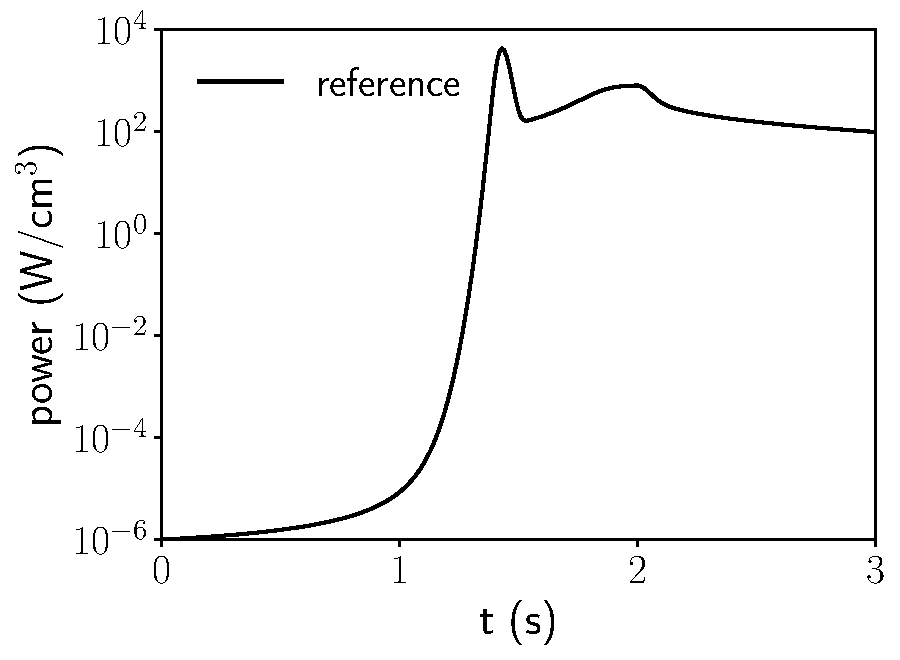
\includegraphics[scale=0.5]{HF_Power.pdf}
\caption{Power from Detran}
\end{figure}
\end{frame}

% \begin{frame}
% \frametitle{Case Study}
% \begin{figure}[ht]
% 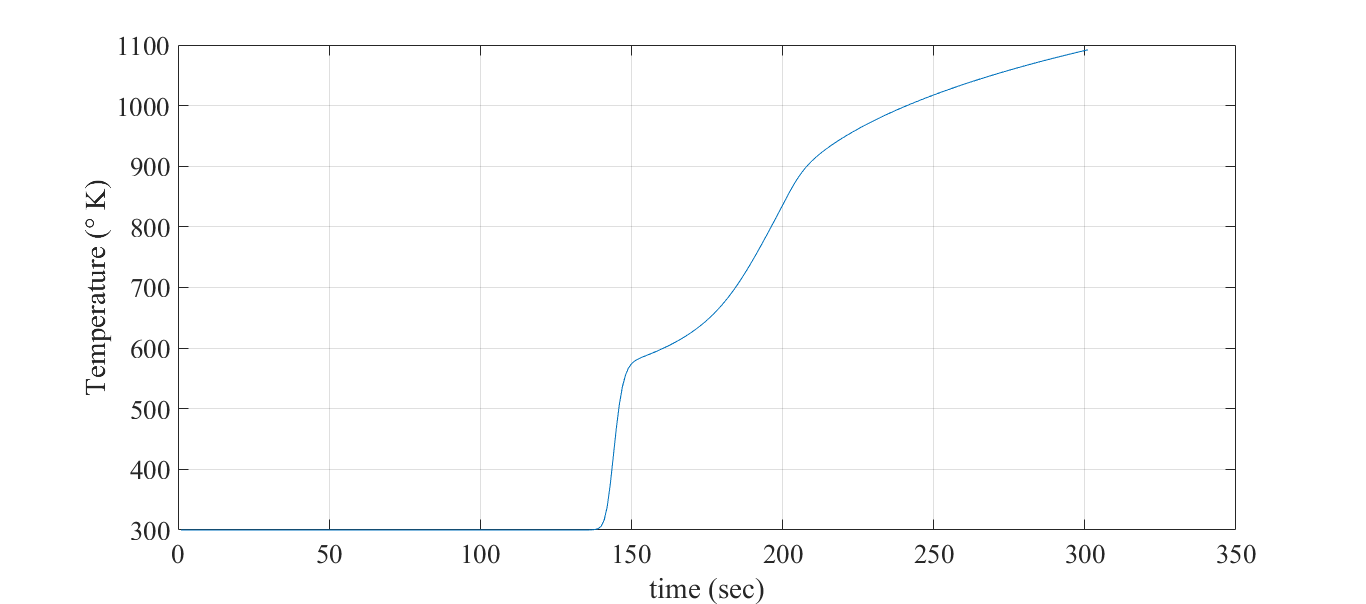
\includegraphics[scale=0.3]{Temp.png}
% \caption{Core Temperature}
% \end{figure}
% \end{frame}

\begin{frame}
\frametitle{Case Study}
\begin{figure}[ht]
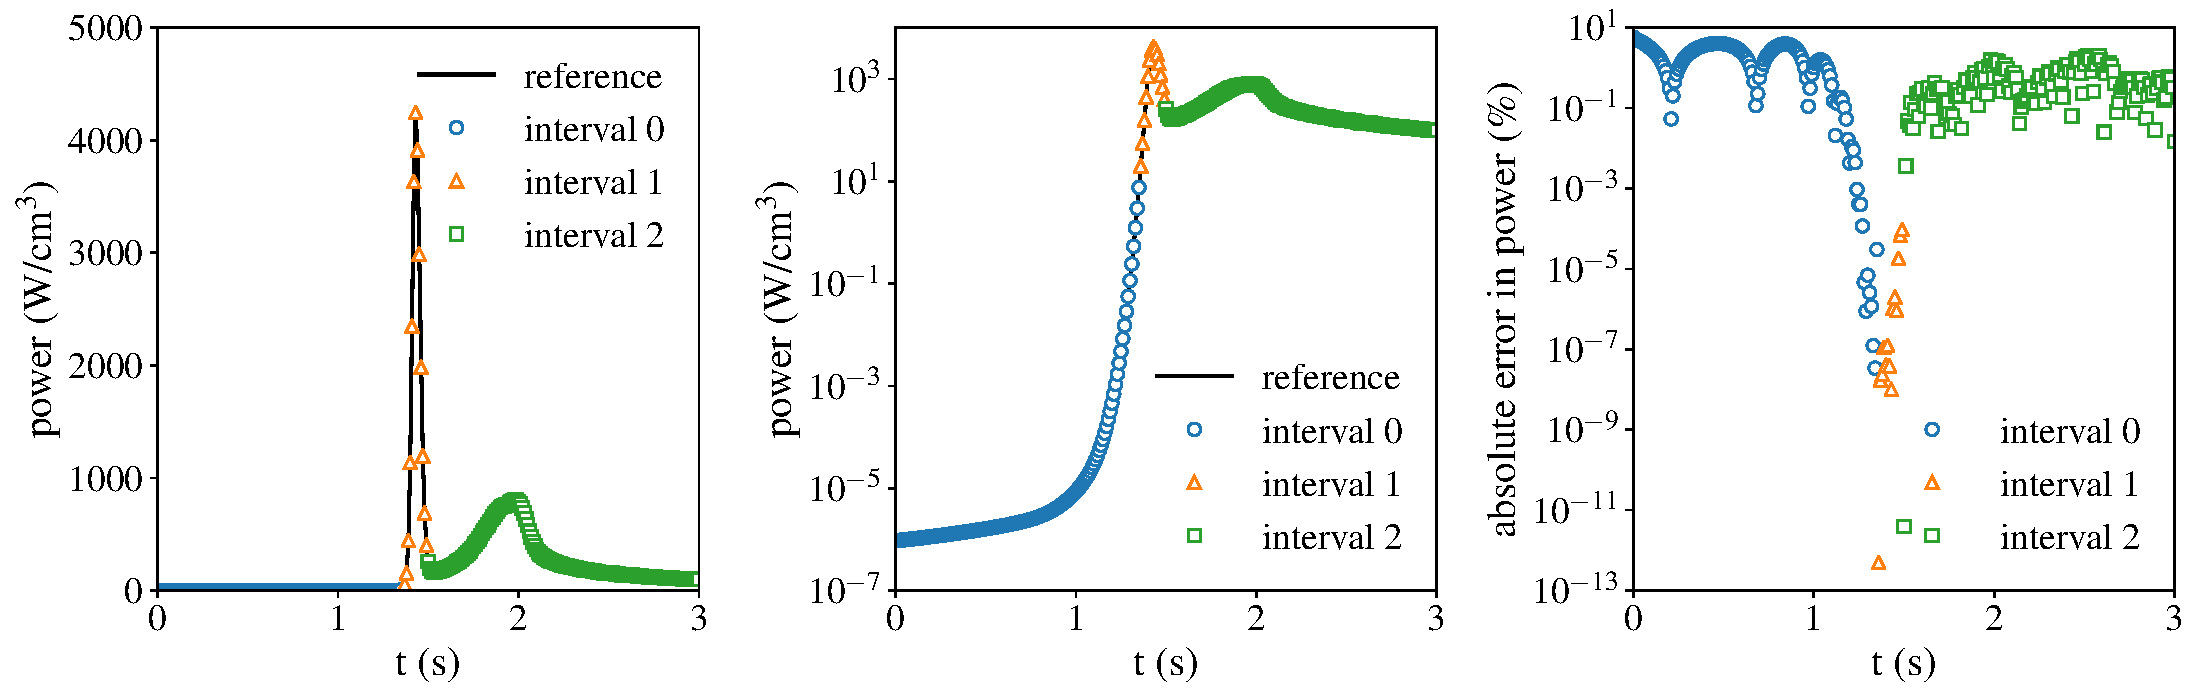
\includegraphics[scale=0.3]{corepower.pdf}
\caption{Partitioned DMD surrogates}
\end{figure}
\end{frame}

\begin{frame}
\frametitle{Case Study}
\begin{figure}[ht]
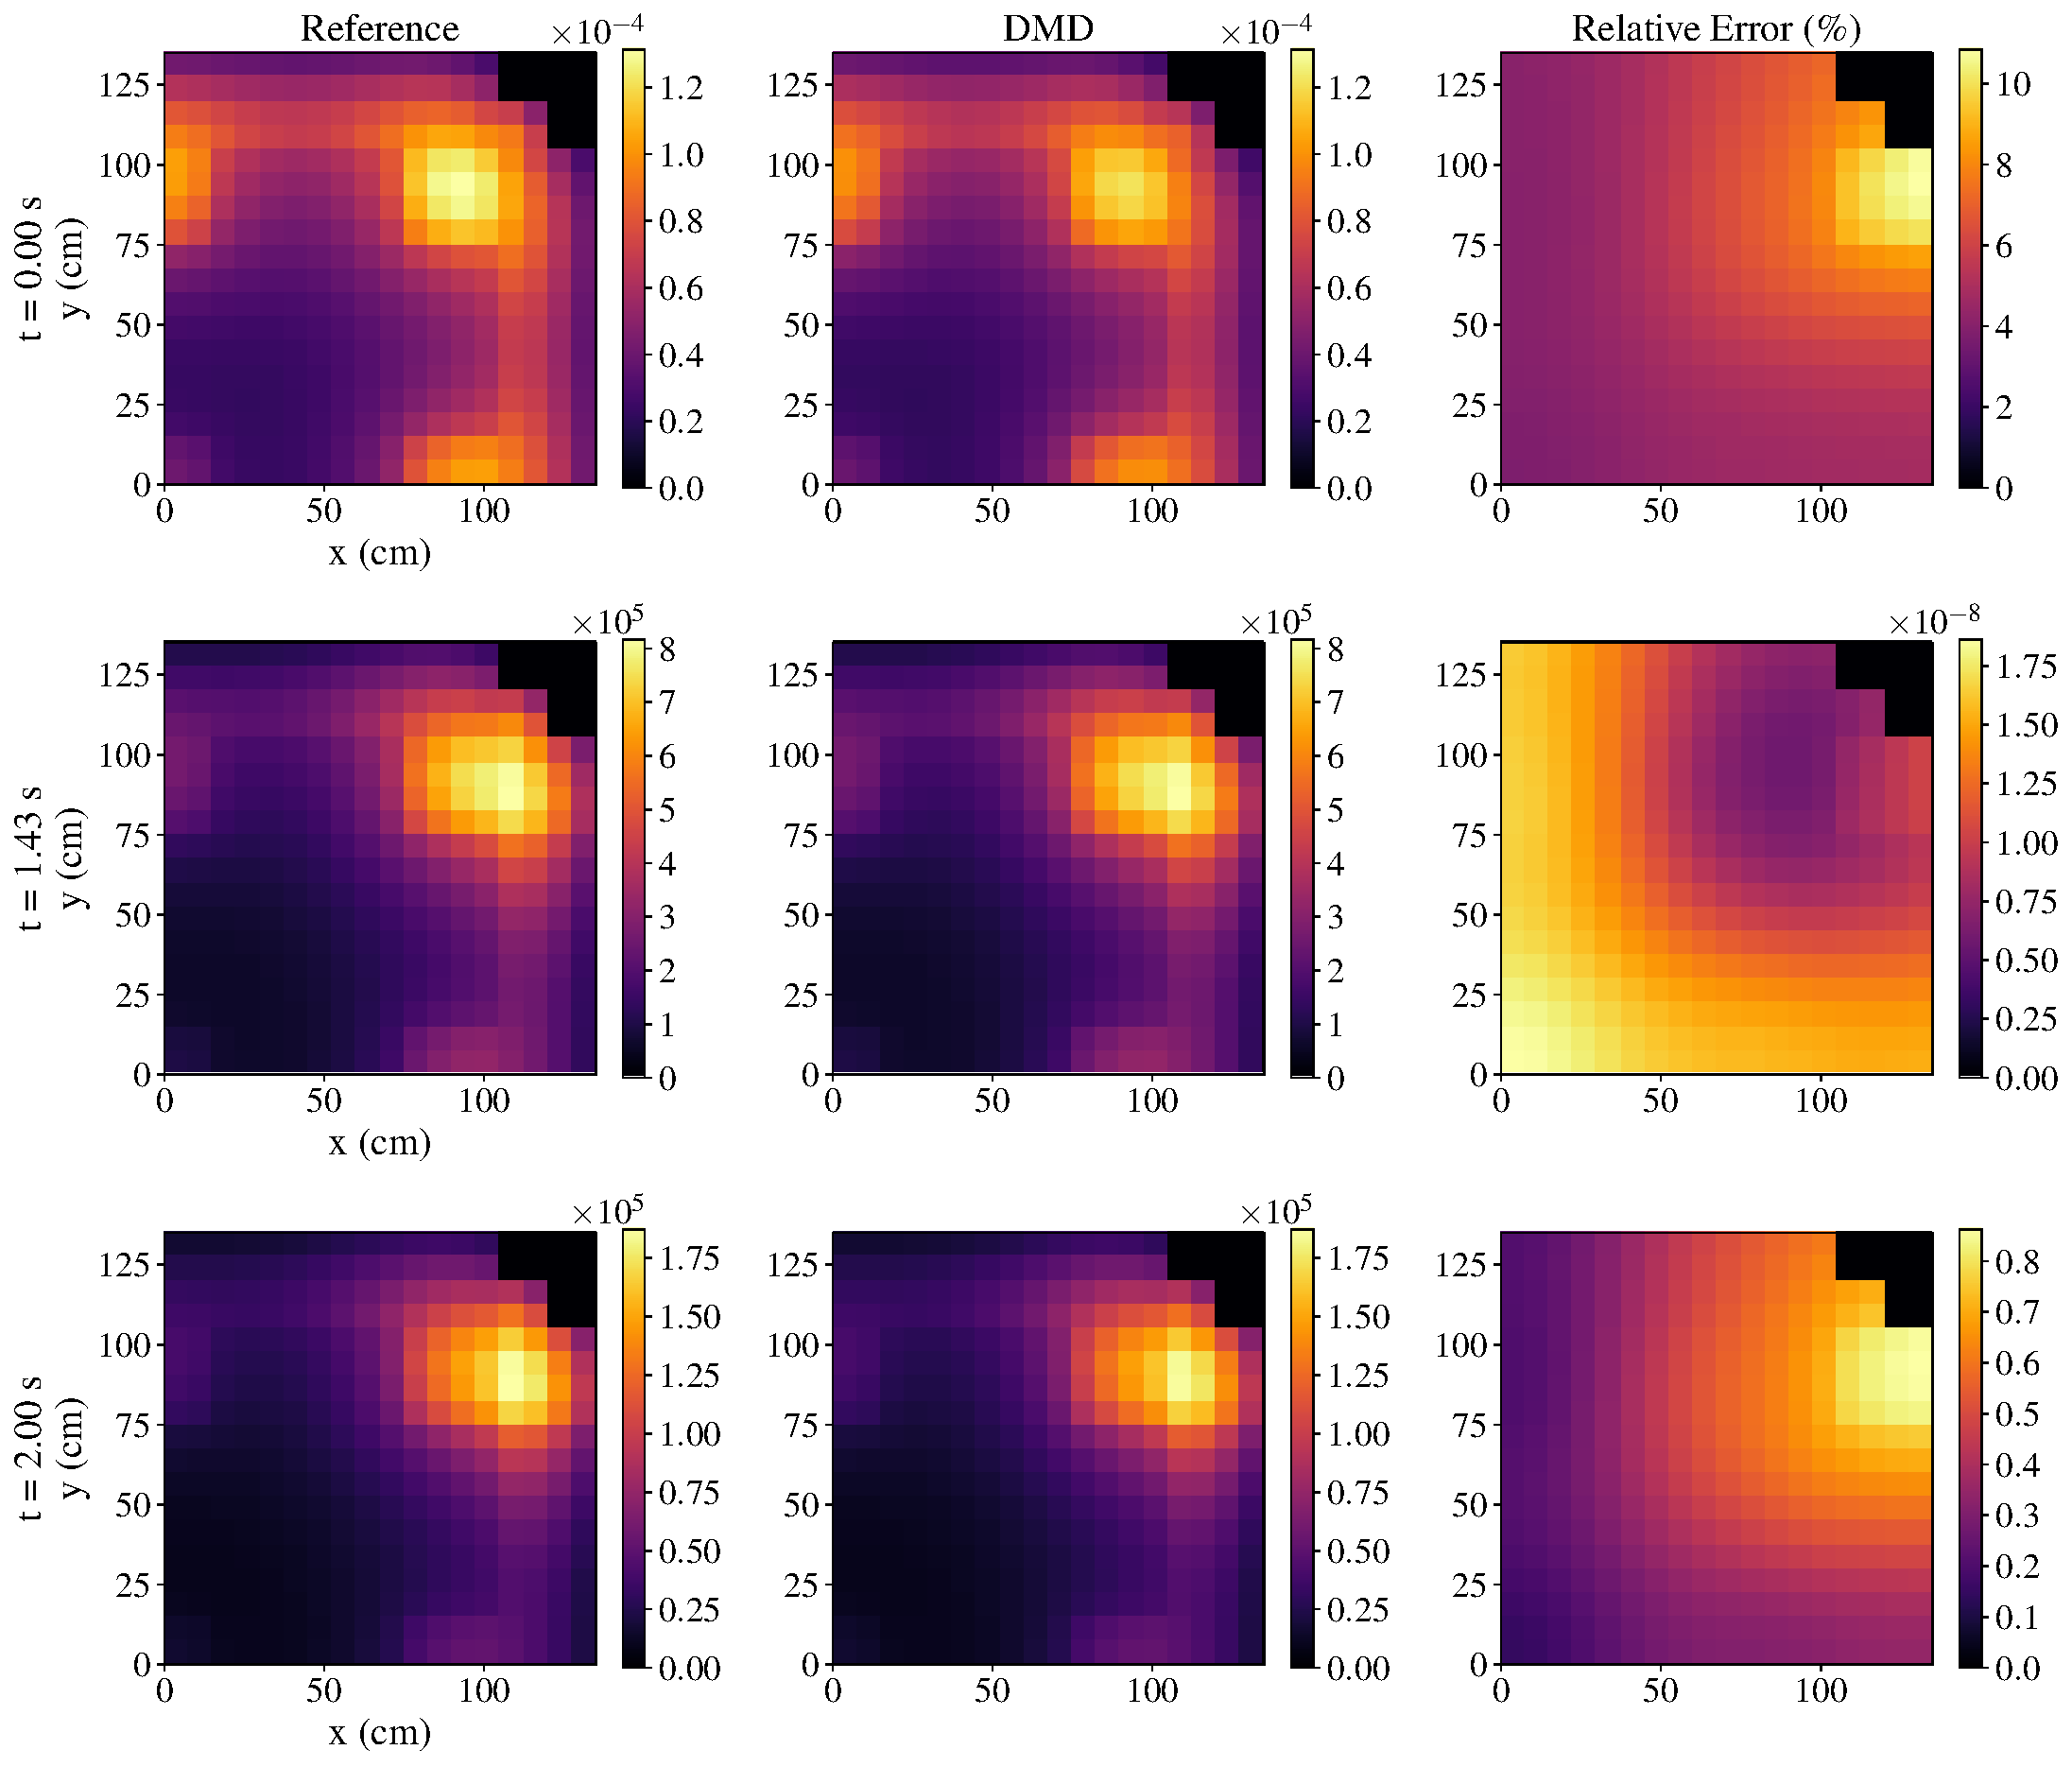
\includegraphics[scale=0.18]{meshpower.pdf}
\caption{Partitioned DMD surrogates}
\end{figure}
\end{frame}

  
   \begin{frame}
   \section{Conclusion and Future Work }
   \frametitle{Conclusion}
   \begin{itemize}
   \item Partitioned DMD surrogate was able to represent the spatio-temporal dynamics of the LRA benchmark.
   \item The benchmark exhibits a rapid severe change in dynamics within a very short time scale.
   \item The surrogate offered a precision of $10^{-8}\%$ in the maximum power region, and a maximum error of 10\% at the very beginning of the simulation. The surrogate was shown to be sensitive to the time partitioning. 
   \item Work is ongoing to mitigate this sensitivity and to provide an automated way to select the number of partitions and their boundaries.
   \end{itemize}
      \end{frame}


    \section{}
%   \section{References}    
    \begin{frame}[t,allowframebreaks]\label{lastframe}
        \frametitle{References}
          \nocite{*}
        \bibliographystyle{ans}
        % make a bibliography.bib file with your references in it
        \bibliography{bibliography}
    \end{frame}
\beginbackup
\begin{frame}{Backup Slides}
\begin{table}[bt]\begin{tabular}{|c|c|} \hline\textbf{POD}& \textbf{DMD}   \\ \hline 
\onslide<1->{\textcolor{green}{Optimality and Orthogonality}}& \onslide<1->{\textcolor{red}{Non-orthogonal}} \\
\onslide<2->{\textcolor{green}{Equations can be injected}}& \onslide<2->{\textcolor{red}{Solely Data-driven}}   \\
\onslide<3->{\textcolor{orange}{Only linear correlations}}& \onslide<3->{\textcolor{green}{captures nonlinearities (Koopman)}}\\
\onslide<4->{\textcolor{red}{Mixed temporal behaviors}}& 
\onslide<4->{\textcolor{green}{explicit temporal frequencies}}\\ 
\onslide<5->$\mathbf{C}=\frac{1}{M}\int_{0}^{\tau} \vec{\phi}(\vec{r},t)\vec{\phi}(\vec{r},t)^T dt$&
\onslide<5-> \\
\onslide<6->{\textcolor{green}{as rank $\uparrow$ error $\downarrow$}}&
\onslide<6->{\textcolor{red}{Optimal rank is a challenge}}\\ \onslide<7->{\textcolor{red}{Modes ordered (energy/variance)}}&
\onslide<7->{\textcolor{orange}{numerous variants/criteria}}\\ 
\hline
\end{tabular}
\end{table}
\end{frame}

\begin{frame}
\frametitle{DMD UQ}
\begin{block}{Sandwich Rule}
\centering
$$\vec{x}^{DMD}(t)=\underbrace{\boldsymbol{\Phi}^{DMD}\mathbf{diag}(e^{\vec{\omega}t})\boldsymbol{\Phi}^{DMD\dagger}}_{\mathbf{S}}\vec{x_0}$$
$$\mathbf{C}_x^{DMD}=\mathbf{S}\mathbf{C}_{0}\mathbf{S}^T,$$
$$\mathbf{C}_{0}=\frac{1}{N-1}\mathbf{X_0}\mathbf{X_0}^T$$
\end{block}
\end{frame}


\backupend

\end{document}
